
\section[Work Flows]{Work Flows}
\label{sec:work_flows}
\addcontentsline{toc}{section}{\thesection. Work Flows}

{\color{red} \bf Warning:}
All work flows are intended to be run in batch mode and on Unix-like systems 
for optimum performance.

The \pkg{cubfits} package is built with some useful work flows,
including
\begin{enumerate}
\item \code{simu} for simulation studies,
\item \code{wphi} for sequences with expression levels ($\phi$) and
                  measurement errors,
\item \code{wophi} for sequences without expression levels, and
\item \code{wphi_wophi} for model validation.
\end{enumerate}
We share these work flows as templates which may be useful for further
research. A quick way to obtain a default work flow is by calling
\code{cubfits::cp.workflow()}, which contains the three aforementioned 
work flows. Note however that these are only tested privately under a 
Linux environment, and are merely served as templates. None of them are 
checked by CRAN.

Figure~\ref{fig:workflows} depicts the analysis process and how \pkg{cubfits}
functions play behind work flows.
\begin{itemize}
\item
input: FASTA file and gene expression for
       ``with'' $\phi$ work flow (\code{wphi}),
\item
execute: major functions \code{cubfits()} and \code{cubappr()} in parallel,
\item
output: save \code{.rda} files for post processing,
\item
post process: subset MCMC iterations and precompute statistics,
\item
diagnosis: generate plots,
\item
summary: obtain parameters for ``with'' $\phi$ work flow, and
\item
feedback: utilize ``with'' $\phi$ results to initial
          ``without'' $\phi$ work flow (\code{wophi}).
\end{itemize}
\begin{figure}[ht]
\centering
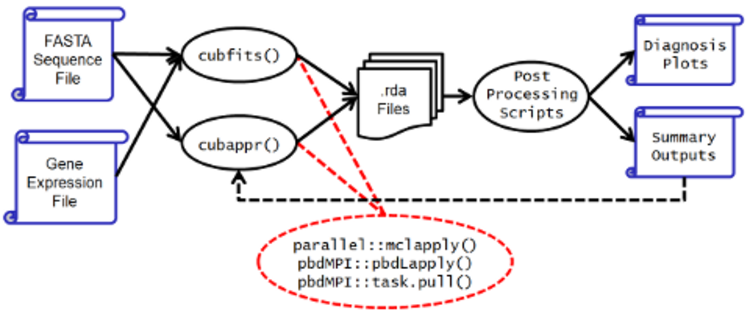
\includegraphics[width=5.5in]{cubfits-include/figure/workflows}
\caption{\code{wphi} work flow is mainly based on \code{cubfits()} and it's
outputs can be initial values for \code{wophi} work flow mainly based on
\code{cubappr()}. Note that \code{wphi} needs both sequence and expression
data, while \code{wophi} only needs sequence. The dashed black line indicate
\code{wphi\_wophi} work flow combining both \code{wphi} and \code{wophi}.
}
\label{fig:workflows}
\end{figure}

The work flows are stored in the package directory
\code{cubfits/inst/workflow/} and installed in
\code{$\{R_HOME\}/library/cubfits/workflow/}. Therefore, executing the
following script can regenerate those work flows in three directories
\code{./01-simu/}, \code{./02-wphi/}, \code{03-wophi} and
\code{./04-wphi\_wophi/}.
\begin{Command}
$ mkdir 01-simu
$ cd 01-simu/
$ Rscript -e "cubfits::cp.workflow('simu')"
$ cd ../
$ mkdir 02-wphi
$ cd 02-wphi/
$ Rscript -e "cubfits::cp.workflow('wphi')"
$ cd ../
$ mkdir 03-wophi
$ cd 03-wophi/
$ Rscript -e "cubfits::cp.workflow('wophi')"
$ cd ../
$ cd 04-wphi_wophi/
$ Rscript -e "cubfits::cp.workflow('wphi_wophi')"
$ cd ../
\end{Command}
Note that a work flow is mainly coded in shell script and sequentially
executes analyses via several shell commands and \proglang{R} scripts. The
analysis \proglang{R} scripts are managed and stored in
\code{cubfits/inst/workflow/} and installed in
\code{$\{R_HOME\}/library/cubfits/workflow/}. Those are served as
templates and can be altered by users (copy scripts to local directory
and modify as needed.)

After regenerating those work flows,
three shell scripts and one \proglang{R} script are created
within each directory.  These scripts consist of:
\begin{itemize}
\item \code{run_0.sh} creates the needed subdirectories,
\item \code{run_1.sh} is the main script of analysis,\footnote{
This may require up to 30 cores and may take a few hours to finish
depending on the number of sequences. Please do some testing and adjust
this file and \code{00-set\_env.r} accordingly before a hero run.
}
\item \code{run_2.sh} is for post processing,
\item \code{run_2_ps.sh} is for post scaling, and
\item \code{00-set_env.r} is the configuration \proglang{R} script
      for \pkg{cubfits}.
\end{itemize}
For \code{simu} work flow, one can sequentially execute those shell scripts
(\code{run_*.sh}) without further changes, and may learn to adjust scripts for 
further studies. For \code{wphi} and \code{wophi} work flows, one needs to 
provide genome sequences (e.g. \code{./02-wphi/param/genome.fasta})
and expression data (e.g. \code{./02-wphi/param/genome.phi.tsv}).

Examples of post processing from the \code{simu} work flow (as in 
(\code{run_2.sh})
are given in Figure~\ref{fig:prxy}. The plots are from files
\code{./01-simu/all.out/plot/prxy_roc_ad_fits_pm_5k-10k.pdf} and \\
\code{./01-simu/all.out/plot/prxy_roc_ad_appr_pm_5k-10k.pdf}.
\begin{figure}[ht]
\centering
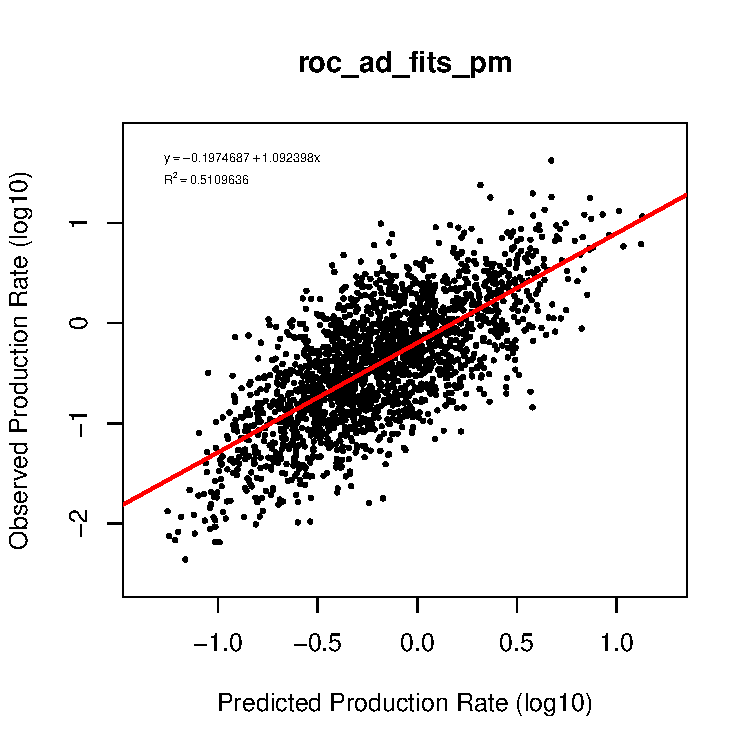
\includegraphics[width=2.75in]{cubfits-include/figure/prxy_roc_ad_fits_pm_5k-10k}
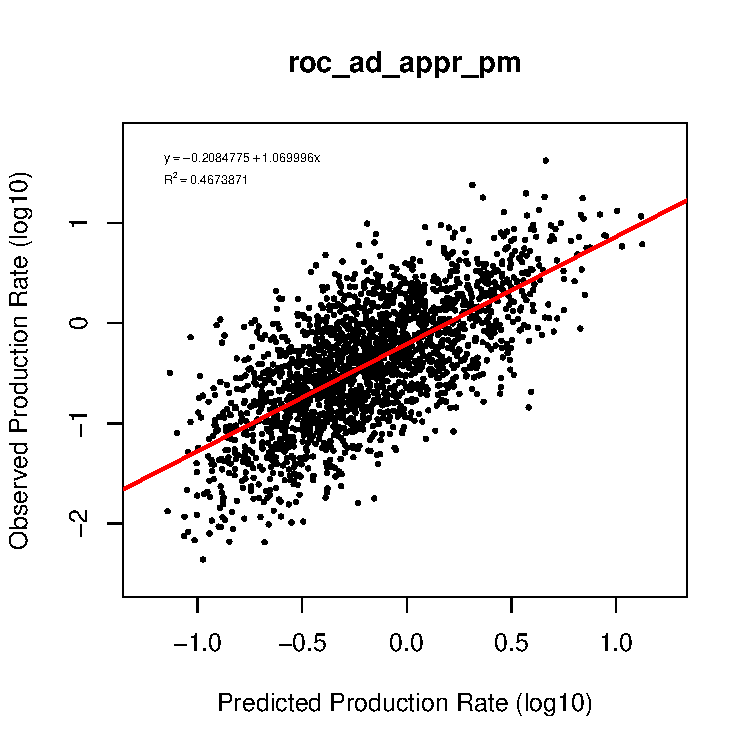
\includegraphics[width=2.75in]{cubfits-include/figure/prxy_roc_ad_appr_pm_5k-10k}
\caption{The left plot is predicted expression (MCMC posterior mean of expected
expression) from model fits against observed
expression (with measurement errors). In the right plot, the predicted
expression is approximated from a simulation (no model fits.)}
\label{fig:prxy}
\end{figure}
